\documentclass[12pt]{article}
\usepackage{graphicx}
%\documentclass[journal,12pt,twocolumn]{IEEEtran}
\usepackage[none]{hyphenat}
\usepackage{graphicx}
\usepackage{listings}
\usepackage[english]{babel}
\usepackage{graphicx}
\usepackage{caption}
\usepackage[parfill]{parskip}
\usepackage{hyperref}
\usepackage{booktabs}
%\usepackage{setspace}\doublespacing\pagestyle{plain}
\def\inputGnumericTable{}
\usepackage{color}                                            %%
    \usepackage{array}                                            %%
    \usepackage{longtable}                                        %%
    \usepackage{calc}                                             %%
    \usepackage{multirow}                                         %%
    \usepackage{hhline}                                           %%
    \usepackage{ifthen}
\usepackage{array}
\usepackage{amsmath}   % for having text in math mode
\usepackage{parallel,enumitem}
\usepackage{listings}
\lstset{
language=tex,
frame=single, 
breaklines=true
}
  
%Following 2 lines were added to remove the blank page at the beginning
\usepackage{atbegshi}% http://ctan.org/pkg/atbegshi
\AtBeginDocument{\AtBeginShipoutNext{\AtBeginShipoutDiscard}}
%
%New macro definitions
\newcommand{\mydet}[1]{\ensuremath{\begin{vmatrix}#1\end{vmatrix}}}
\providecommand{\brak}[1]{\ensuremath{\left(#1\right)}}
\providecommand{\norm}[1]{\left\lVert#1\right\rVert}
\newcommand{\solution}{\noindent \textbf{Solution: }}
\newcommand{\myvec}[1]{\ensuremath{\begin{pmatrix}#1\end{pmatrix}}}
\let\vec\mathbf
\begin{document}
\begin{center}
\title{\textbf{Straight Lines}}
\date{\vspace{-5ex}} %Not to print date automatically
\maketitle
\end{center}
\setcounter{page}{1}
\section*{11$^{th}$ Maths - Chapter 10}
This is Problem-8 from Exercise 10.3
\begin{enumerate}
	\item Find the equation of line perpendicular to the line $x-7y+5=0$ and having $x$ intercept $3$.\\
\solution
Given line is 
\begin{align}
	x-7+5=0
\end{align}
A line equation can be expressed as 
\begin{align}
	\vec{n}^{\top}\vec{x}=c
\end{align}
\begin{align}
	\text{ where }
		\vec{n} = \myvec{1\\-7} , c = -5
\end{align}
the equation of line which is perpendicular with a  $x$ intercept $3$ is given by 
\begin{align}
	\vec{m}^\top\brak{\vec{x}-\vec{A}}=0 \label{eq:4}
\end{align}
		here $\vec{m}$ and $\vec{A}$ are 
\begin{align}
	\vec{m} &=\myvec{7\\1}\\
	\vec{m}^\top &=\myvec{7 & 1}\\
	\vec{A} &=\myvec{3\\0}
\end{align}
		Substituting the value of $\vec{m}$ and $\vec{A}$ in \eqref{eq:4}
		\begin{align}
			\myvec{7 & 1}\brak{\vec{x}-\myvec{3\\0}} &=0\\
			\myvec{7 & 1}\vec{x}-21 &=0\\
			\myvec{7 & 1}\vec{x} &= 21
		\end{align}
\begin{figure}[!h]
\begin{center}
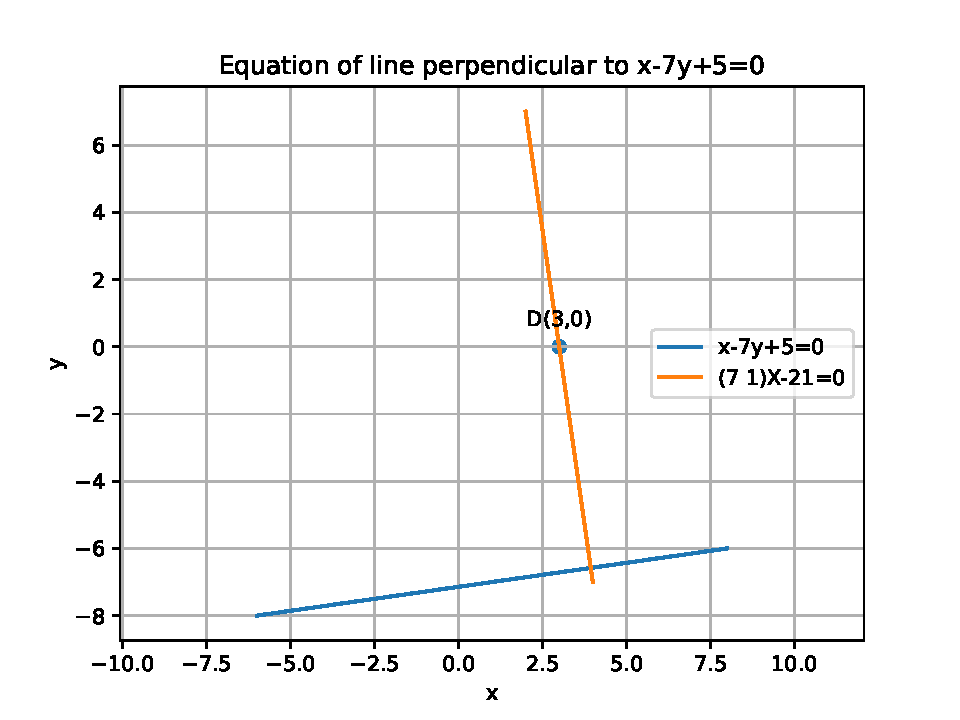
\includegraphics[width=\columnwidth]{figs/fig.pdf}
\end{center}
\caption{}
\label{fig:Fig1}
\end{figure}
\end{enumerate}
\end{document}